%% Báo cáo tiếng Việt -- Elsevier CAS single-column (cas-sc)
\documentclass[a4paper,fleqn]{cas-sc}

\usepackage[utf8]{inputenc}
\usepackage[T5]{fontenc}
\usepackage[vietnamese]{babel}

\usepackage[numbers,sort&compress]{natbib}
\usepackage{amsmath,amssymb}
\usepackage{booktabs}
\usepackage{graphicx}
\usepackage{multirow}
\usepackage{xcolor}
\usepackage{lastpage}

\AtBeginDocument{\def\lastpage{\csname lastpage@lastpage\endcsname}}

\graphicspath{{../figures/}}

\shorttitle{Mã hoá SAT cho N-Queens}
\shortauthors{T.Đ. Đức}

\begin{document}
\let\WriteBookmarks\relax
\def\floatpagepagefraction{1}
\def\textpagefraction{.001}

\title[mode=title]{Mã hoá SAT chính xác cho bài toán N-Queens:\newline
So sánh thực nghiệm với MIP và CP}

\author[1]{Trương Đình Đức}

\affiliation[1]{organization={Khoa Công nghệ Thông tin,
  Trường Đại học Công nghệ, Đại học Quốc gia Hà Nội},
  city={Hà Nội}, postcode={100000}, country={Việt Nam}}

\begin{abstract}
Bài toán N-Queens yêu cầu đặt $n$ quân hậu không ăn nhau trên bàn cờ $n\times n$
và là một bài kiểm thử kinh điển cho các phương pháp giải tổ hợp. Chúng tôi trình
bày một phương pháp mã hoá SAT chính xác cho N-Queens thông qua các ràng buộc
đếm ``nhiều nhất một'' (at-most-one, AMO) và ``ít nhất một'' (at-least-one,
ALO), đồng thời nghiên cứu sự tương tác giữa cách mã hoá đếm và lựa chọn bộ giải
SAT. Chúng tôi tự cài đặt năm cách mã hoá (pairwise, binary, commander, product,
sequential) và sử dụng bảy cách mã hoá có sẵn trong thư viện PySAT, rồi đánh giá
tám bộ giải SAT trên các instance từ $n=8$ đến $n=80$ (lặp ba lần, giới hạn thời
gian 600\,giây). Phương pháp SAT được so sánh với bảy baseline chính xác xây dựng
bằng Gurobi, CPLEX (MIP và CP), OR-Tools CP-SAT, OR-Tools MIP (backend SCIP) và
PuLP/CBC. Kết quả cho thấy tương tác mạnh giữa encoding và solver: cách mã hoá
pairwise là bền vững nhất và chiếm ưu thế với các solver yếu, trong khi cách mã
hoá binary nhanh nhất với các solver mạnh. MiniSat và MiniCard là hai bộ giải SAT
hiệu quả nhất nói chung, còn Glucose bị timeout ở những encoding khó. Trong số
các baseline, Gurobi nhanh nhất vượt trội với thời gian gần như không đổi, CPLEX
MIP đứng thứ hai; cấu hình SAT tốt nhất ngang ngửa CP-SAT và CPLEX CP nhưng chậm
hơn rõ rệt so với hai bộ giải MIP thương mại trên bài toán mang tính khả thi này.
\end{abstract}

\begin{keywords}
N-Queens \sep mã hoá SAT \sep ràng buộc đếm \sep AMO \sep PySAT \sep
MIP \sep quy hoạch ràng buộc \sep đánh giá thực nghiệm
\end{keywords}

\maketitle

\section{Giới thiệu}\label{sec:intro}
Bài toán N-Queens là bài toán đặt $n$ quân hậu trên bàn cờ $n\times n$ sao cho
không có hai quân hậu nào ăn nhau, tức là không có hai quân cùng hàng, cùng cột
hoặc cùng đường chéo. Đây là bài toán thoả mãn ràng buộc nổi tiếng, đã được
nghiên cứu trong nhiều thập kỷ cả về cấu trúc tổ hợp lẫn như một benchmark cho
các thuật toán chính xác và heuristic \citep{BellStevens2009}. Mặc dù sự tồn tại
nghiệm được biết với mọi $n \geq 4$, việc tìm một cách đặt thoả mãn và so sánh
hiệu năng của các công nghệ giải chính xác khác nhau vẫn là một nghiên cứu tình
huống hữu ích.

Các bộ giải thoả mãn logic mệnh đề (SAT) hiện đại, dựa trên học mệnh đề từ xung
đột (CDCL) \citep{MarquesSilva1999}, đã trở thành công cụ hiệu quả cho nhiều bài
toán tổ hợp. Câu đố N-Queens có thể được mã hoá thành dạng chuẩn hội (CNF) bằng
cách biểu diễn mỗi ô cờ bởi một biến Boolean và biểu diễn các ràng buộc ăn nhau
cùng điều kiện ``mỗi hàng đúng một quân hậu'' dưới dạng các ràng buộc đếm. Hiệu
quả của CNF thu được phụ thuộc mạnh vào cách mã hoá ràng buộc AMO và ALO
\citep{Sinz2005,Prestwich2009,KlieberKwon2007}.

Trong bài báo này, chúng tôi đặt câu hỏi: cách mã hoá đếm tương tác với bộ giải
SAT như thế nào, và SAT so với các phương pháp chính xác khác như Quy hoạch
nguyên hỗn hợp (MIP) và Quy hoạch ràng buộc (CP) ra sao trên bài toán N-Queens.
Các đóng góp của chúng tôi gồm:
\begin{itemize}
  \item Cài đặt năm cách mã hoá AMO từ đầu (pairwise, binary, commander, product
        và sequential của Sinz) và dùng bảy cách mã hoá của thư viện PySAT, tất cả
        trong một package Python dùng lại được.
  \item Đánh giá tám bộ giải SAT (MiniSat, MiniCard, CaDiCaL 1.5.3 và 1.9.5,
        MergeSAT, Lingeling, Glucose 3 và 4) trên các instance từ $n=8$ đến
        $n=80$ với ba lần lặp và giới hạn thời gian 600\,giây.
  \item So sánh SAT với bảy baseline chính xác dựng bằng Gurobi, CPLEX (MIP và
        CP), OR-Tools CP-SAT, OR-Tools MIP (backend SCIP) và PuLP (backend CBC).
  \item Báo cáo và thảo luận về tương tác mạnh giữa encoding và solver, một hiện
        tượng đặc thù của tiền xử lý của bộ giải, và khoảng cách giữa SAT với các
        bộ giải MIP/CP thương mại trên bài toán này.
\end{itemize}

Phần còn lại của bài báo được tổ chức như sau. Mục~\ref{sec:background} định
nghĩa bài toán, điểm lại các cách mã hoá ràng buộc đếm và trình bày các nghiên
cứu liên quan. Mục~\ref{sec:method} trình bày mô hình CNF, các encoding, khung
giải và các baseline. Mục~\ref{sec:experiments} báo cáo thực nghiệm và thảo luận
kết quả. Mục~\ref{sec:conclusion} kết luận.

\section{Cơ sở lý thuyết}\label{sec:background}

\subsection{Định nghĩa bài toán và mô hình CNF}
Gọi $x_{r,c}$ là biến Boolean đúng khi và chỉ khi có quân hậu tại hàng $r$, cột
$c$, với $0 \leq r,c < n$, do đó dùng $n^2$ biến. Một cách đặt hợp lệ phải thoả
các ràng buộc sau:
\begin{align}
  \sum_{c=0}^{n-1} x_{r,c} &= 1 && \forall r \quad \text{(đúng một quân mỗi hàng)},\\
  \sum_{r=0}^{n-1} x_{r,c} &\leq 1 && \forall c \quad \text{(nhiều nhất một quân mỗi cột)},\\
  \sum_{\substack{(r,c)\in D}} x_{r,c} &\leq 1 && \forall \text{đường chéo } D ,
\end{align}
trong đó một đường chéo là tập hợp ô cờ tối đa có $r-c$ không đổi (đường chéo
chính) hoặc $r+c$ không đổi (đường chéo phụ). Vì mỗi hàng chứa đúng một quân
hậu nên có đúng $n$ quân hậu; do đó ràng buộc cột và đường chéo chỉ cần chiều
``nhiều nhất một''. Điều kiện đúng-một của hàng được mã hoá bằng hội của một
ràng buộc ALO và một ràng buộc AMO, còn cột và đường chéo chỉ cần AMO.

\subsection{Các cách mã hoá ràng buộc đếm}
Ràng buộc AMO trên các literal $\ell_1,\dots,\ell_m$ phát biểu rằng nhiều nhất
một literal đúng, còn ALO phát biểu rằng ít nhất một literal đúng. Chúng tôi xét
các cách mã hoá AMO sau, với $m$ là số literal.
\begin{itemize}
  \item \textbf{Pairwise.} Một mệnh đề $(\neg \ell_i \vee \neg \ell_j)$ cho mỗi
        cặp không thứ tự $\{i,j\}$: $\binom{m}{2}$ mệnh đề, không có biến phụ.
        Lan truyền mạnh nhưng CNF lớn.
  \item \textbf{Binary.} Mỗi literal được gán một mã nhị phân gồm
        $\lceil \log_2 m \rceil$ bit phân biệt và các kéo theo cưỡng chế mã; dùng
        $m\lceil\log_2 m\rceil$ mệnh đề và $\lceil\log_2 m\rceil$ biến phụ.
  \item \textbf{Commander.} Các literal được chia thành nhóm kích thước tối đa
        $g$; mỗi nhóm có một biến commander, AMO được áp trong từng nhóm và giữa
        các commander theo đệ quy. Cách này giảm số mệnh đề xuống $O(m)$ với chi
        phí thêm biến.
  \item \textbf{Product.} Các literal được xếp trên lưới $p\times q$ ($pq \geq
        m$); các kéo theo liên hệ mỗi literal với một biến hàng và một biến cột,
        và AMO được áp trên các biến hàng, biến cột.
  \item \textbf{Sequential (Sinz).} Một chuỗi $m-1$ biến phụ mã hoá ``số literal
        đúng đã gặp nhiều nhất là một'', dùng $3m-4$ mệnh đề và $m-1$ biến phụ;
        đây là cách mã hoá bộ đếm tuần tự tiêu chuẩn \citep{Sinz2005}.
\end{itemize}
Ngoài ra, PySAT \citep{Ignatiev2018} cung cấp các cách mã hoá \emph{bitwise},
\emph{ladder}, \emph{sorting-network}, \emph{cardinality-network} và
\emph{totalizer}, được đưa vào để đầy đủ. Số biến và số mệnh đề của mỗi encoding
với $n=40$ được báo cáo ở Bảng~\ref{tab:structure}.

\subsection{Nghiên cứu liên quan}
N-Queens có lịch sử lâu dài trong tổ hợp \citep{BellStevens2009}, và phiên bản
quyết định của nó (N-Queens Completion) đã được chứng minh là NP-đầy đủ
\citep{Gent2017}, điều này tạo động lực cho các bộ giải chính xác tổng quát. Về
phía SAT, mã hoá ràng buộc đếm là chủ đề trung tâm trong Handbook of
Satisfiability \citep{Biere2021,Prestwich2009}, với bộ đếm tuần tự của Sinz
\citep{Sinz2005}, các cách dựng pairwise và commander
\citep{KlieberKwon2007}, và các biến thể binary và product
\citep{FrischGiannaros2010} được dùng phổ biến nhất. PySAT \citep{Ignatiev2018}
cung cấp các encoding này qua một giao diện thống nhất, và các solver CDCL hiện
đại như MiniSat \citep{EenSorensson2003}, Glucose \citep{AudemardSimon2009} và
CaDiCaL/Kissat \citep{Biere2020} mang lại động cơ tìm kiếm mạnh. Về phía tối ưu,
các bộ giải MIP và CP như Gurobi \citep{Gurobi2024}, CPLEX \citep{IBM2022},
OR-Tools \citep{ORtools2023} và CBC \citep{ForrestCBC} là các baseline chính xác
tiêu chuẩn. Nghiên cứu của chúng tôi kết nối các hướng này bằng cách so sánh có
hệ thống các encoding đếm, các bộ giải SAT và các baseline MIP/CP trên cùng một
mô hình N-Queens.

\section{Phương pháp}\label{sec:method}

\subsection{Xây dựng mô hình}
Chúng tôi dựng CNF với hàng được mã hoá dạng đúng-một (ALO + AMO), còn cột và
đường chéo được mã hoá dạng AMO như đã mô tả ở Mục~\ref{sec:background}. Các biến
gốc chiếm các định danh $1,\dots,n^2$ và biến phụ được cấp phát sau đó. Có hai
cách mã hoá đường chéo: chế độ \emph{naive} thêm mệnh đề pairwise
$(\neg x_{r_1,c_1} \vee \neg x_{r_2,c_2})$ cho mọi cặp ô cùng đường chéo (bùng nổ
bậc hai trên mỗi đường chéo), và chế độ \emph{optimal} áp encoding AMO đã chọn
một lần cho mỗi đường chéo, giữ số đường chéo tuyến tính và tái dùng cùng một bộ
mã hoá.

\subsection{Encoding và bộ giải}
Năm cách mã hoá tự viết và bảy cách mã hoá của PySAT dùng chung một giao diện, do
đó cùng một mô hình có thể được khởi tạo với bất kỳ encoding nào. Việc giải được
thực hiện qua PySAT; mỗi lần giải chạy trong một tiến trình con tách biệt để một
solver bị crash hoặc treo được ghi nhận là \texttt{crash} hoặc \texttt{timeout}
thay vì làm hỏng cả thực nghiệm. Với mỗi lần chạy, chúng tôi ghi lại thời gian
dựng CNF, thời gian giải, số biến, số mệnh đề và thống kê của solver (số quyết
định, số lan truyền, số xung đột).

\subsection{Các baseline MIP/CP}
Cùng mô hình N-Queens được biểu diễn với các biến nhị phân $a_{r,c}$ thoả đúng-một
mỗi hàng, nhiều nhất-một mỗi cột và nhiều nhất-một mỗi đường chéo, dùng các engine
sau: Gurobi \citep{Gurobi2024}, CPLEX MIP và CPLEX CP \citep{IBM2022}, OR-Tools
CP-SAT \citep{ORtools2023}, OR-Tools MIP với backend SCIP, và PuLP với backend CBC
\citep{ForrestCBC}. Tất cả baseline cực tiểu hoá hàm mục tiêu hằng (bài toán là
bài toán khả thi) và chạy dưới cùng giới hạn thời gian như các bộ giải SAT.

\section{Thực nghiệm}\label{sec:experiments}

\subsection{Thiết lập thực nghiệm}
Tất cả thực nghiệm chạy trên máy Windows với bộ xử lý Intel thế hệ thứ 11, dùng
Python 3.11 và PySAT 1.8/1.9. Chúng tôi dùng các bộ giải SAT MiniSat
(\texttt{minisat22}), MiniCard (\texttt{minicard}), CaDiCaL 1.5.3 và 1.9.5,
MergeSAT 3, Lingeling, và Glucose 3 và 4. Các instance từ $n=8$ đến $n=80$ với
bước hai. Mỗi cấu hình được lặp ba lần và báo cáo giá trị trung vị; giới hạn thời
gian là 600\,giây mỗi lần chạy. Hai bộ giải PySAT có trên một số nền tảng
(\texttt{cryptosat}, \texttt{minisatgh}) không có trong bản phân phối dùng ở đây,
và \texttt{kissat404} tái hiện crash trên các instance này; do đó các solver này
bị loại. Mọi instance được báo cáo đều thoả mãn, nên chúng tôi đo thời gian
\emph{tìm} một mô hình chứ không phải chứng minh vô nghiệm.

\subsection{Cấu trúc CNF}
Bảng~\ref{tab:structure} cho thấy kích thước CNF của mỗi encoding với $n=40$. Cách
mã hoá pairwise dùng ít biến nhất (chỉ $n^2$ biến gốc) nhưng nhiều mệnh đề nhất,
trong khi cách sequential dùng nhiều biến nhất và tương đối ít mệnh đề. Các cách
commander và product cần ít mệnh đề hơn binary nhưng thêm nhiều biến phụ.

\begin{table}[t]
\centering
\caption{Kích thước CNF của mỗi encoding với n = 40.}
\label{tab:structure}
\begin{tabular}{lrr}
\toprule
encoding & \#vars & \#clauses \\
\midrule
pairwise & 1600 & 103520 \\
binary & 2776 & 35584 \\
commander & 4668 & 18006 \\
product & 4042 & 18516 \\
sequential & 7762 & 18292 \\
\bottomrule
\end{tabular}
\end{table}


\subsection{Các bộ giải SAT và encoding}
Bảng~\ref{tab:solver_rank} xếp hạng các bộ giải SAT theo thời gian trung vị trên
mọi encoding với $n\geq 40$, cùng số lần timeout. MiniSat và MiniCard nhanh và bền
vững nhất, tiếp theo sát là hai phiên bản CaDiCaL; Glucose 3 và 4 chậm hơn đáng kể
và là những solver duy nhất bị timeout.

\begin{table}[t]
\centering
\caption{Xếp hạng các bộ giải SAT với $n \geq 40$ (thời gian trung vị trên mọi encoding) và số lần timeout.}
\label{tab:solver_rank}
\begin{tabular}{lrr}
\toprule
solver & median time (s) & timeouts \\
\midrule
minisat22 & 0.421 & 0 \\
minicard & 0.428 & 0 \\
cadical153 & 1.358 & 0 \\
cadical195 & 1.518 & 0 \\
mergesat3 & 1.871 & 0 \\
lingeling & 2.168 & 0 \\
glucose4 & 19.373 & 13 \\
glucose3 & 27.532 & 80 \\
\bottomrule
\end{tabular}
\end{table}


Bảng~\ref{tab:enc_solver} và Hình~\ref{fig:heatmap} cho thấy thời gian trung vị
như hàm của cả encoding lẫn solver, bộc lộ tương tác mạnh giữa
\emph{encoding--solver}: không có encoding nào chiếm ưu thế tuyệt đối. Cách mã hoá
pairwise đồng đều nhanh (khoảng $0{,}6$--$0{,}8$\,giây với mọi solver), trong khi
binary là lựa chọn tốt nhất cho MiniSat và MiniCard ($0{,}19$--$0{,}21$\,giây)
nhưng tệ hơn hẳn với Glucose (tới $48{,}9$\,giây). Các encoding product và
commander là yếu nhất với Glucose, vượt $200$\,giây.

\begin{table}[t]
\centering
\caption{Thời gian giải SAT trung vị (giây) với $n \geq 40$ theo encoding và solver (-- = mọi lần chạy đều timeout).}
\label{tab:enc_solver}
\begin{tabular}{lrrrrrrrr}
\toprule
encoding & minisat22 & minicard & cadical153 & cadical195 & mergesat3 & lingeling & glucose4 & glucose3 \\
\midrule
pairwise & 0.599 & 0.621 & 0.945 & 0.949 & 0.591 & 0.583 & 0.775 & 0.810 \\
binary & 0.192 & 0.205 & 1.056 & 0.949 & 0.819 & 1.796 & 16.887 & 48.854 \\
commander & 0.598 & 0.611 & 1.039 & 1.299 & 5.328 & 20.168 & 47.784 & 203.359 \\
product & 0.461 & 0.467 & 2.120 & 2.080 & 1.871 & 13.433 & 20.317 & 291.456 \\
sequential & 0.482 & 0.476 & 2.048 & 2.594 & 4.121 & 1.552 & 25.639 & 30.234 \\
\bottomrule
\end{tabular}
\end{table}


\begin{figure}[t]
  \centering
  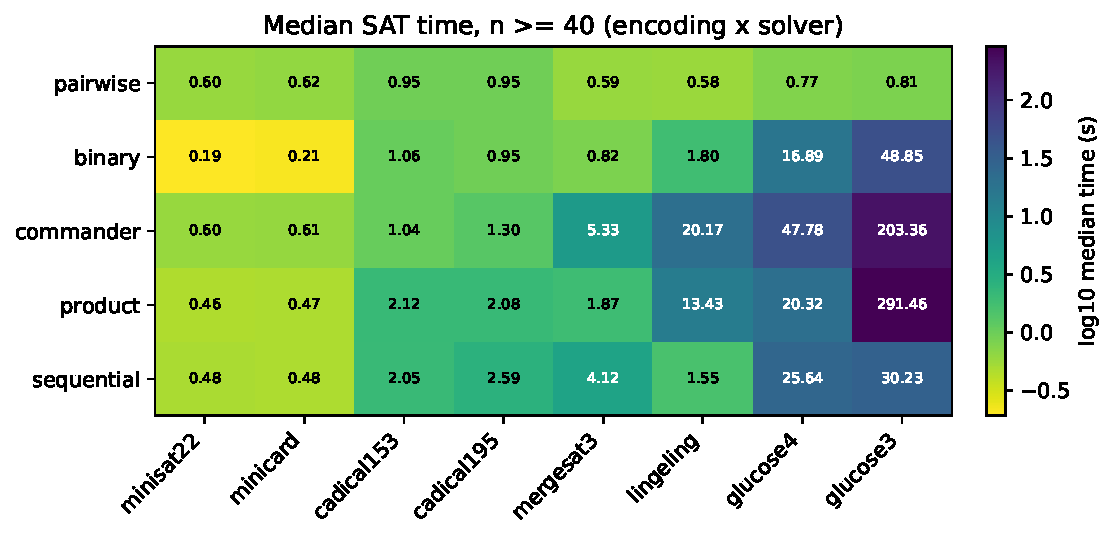
\includegraphics[width=\linewidth]{heatmap_encoding_solver}
  \caption{Thời gian giải SAT trung vị ($n\geq 40$) cho từng cặp
  encoding--solver; ô càng đậm càng chậm. Ô trống ứng với cấu hình mà mọi lần
  chạy đều timeout.}
  \label{fig:heatmap}
\end{figure}

Hình~\ref{fig:by_encoding} biểu diễn thời gian như hàm của $n$ cho từng encoding
với một đường ứng với mỗi solver. Các đường của pairwise bám sát nhau, thể hiện
tính bền vững qua các solver, còn các encoding khác phân kỳ mạnh khi $n$ tăng, với
các đường Glucose vọt lên cao hơn nhiều bậc độ lớn.

\begin{figure*}[t]
  \centering
  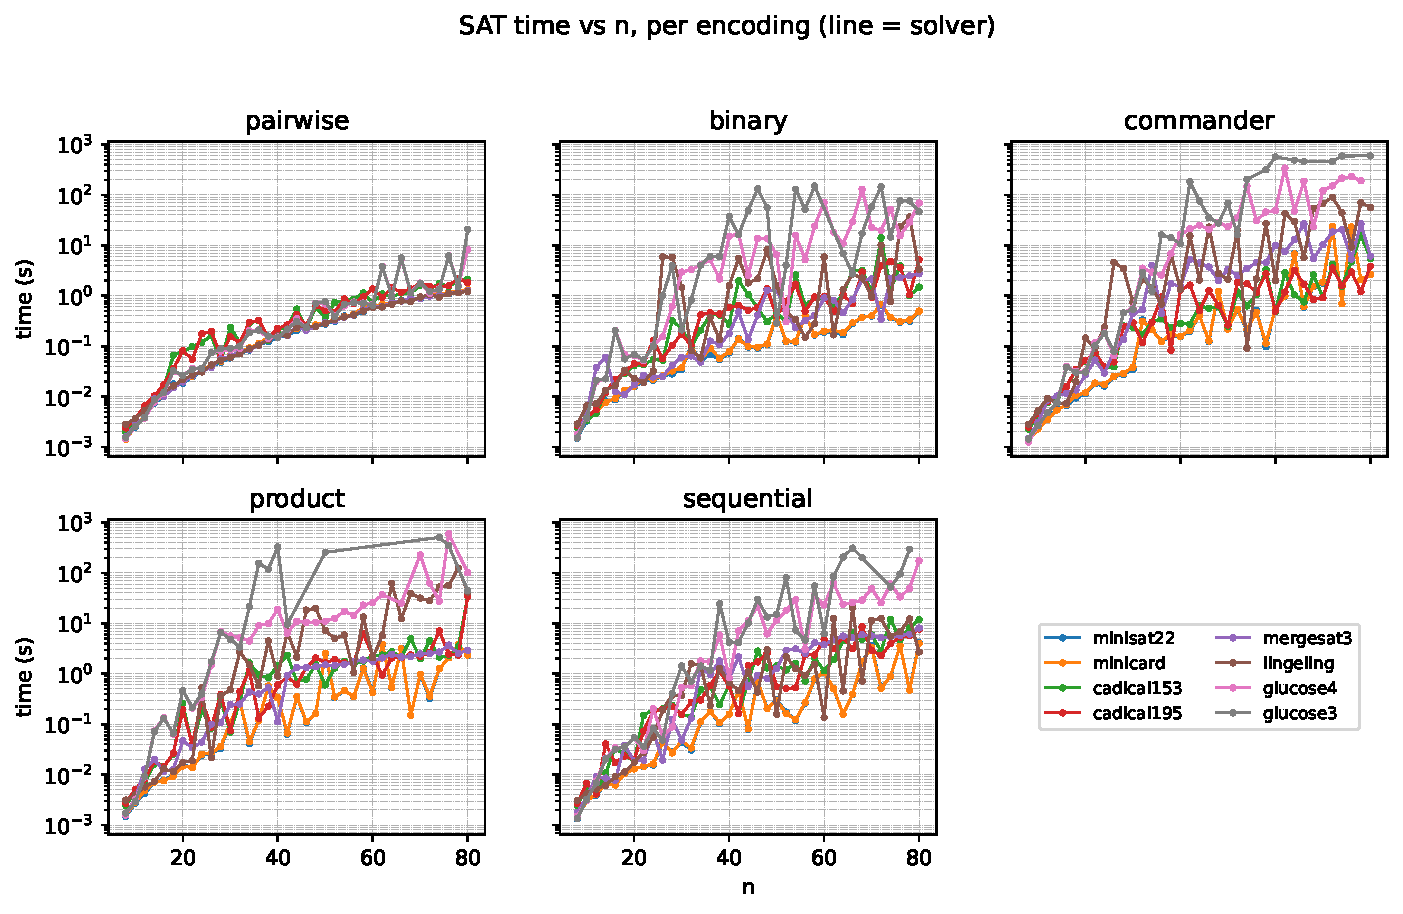
\includegraphics[width=\textwidth]{solver_by_encoding}
  \caption{Thời gian giải SAT theo $n$ cho mỗi encoding (đường = solver). Ô
  pairwise đồng đều nhất; các ô còn lại tách rõ solver mạnh và solver yếu.}
  \label{fig:by_encoding}
\end{figure*}

\subsection{So sánh với MIP và CP}
Bảng~\ref{tab:baseline} và Hình~\ref{fig:baselines} báo cáo các baseline MIP/CP.
Gurobi nhanh nhất vượt trội, thời gian gần như không đổi khoảng $0{,}005$\,giây bất
kể $n$; CPLEX MIP đứng thứ hai với khoảng $0{,}1$\,giây ở $n=80$. CP-SAT và
CPLEX CP tăng rõ hơn, còn các baseline MIP dùng SCIP và CBC chậm và nhiễu hơn.

\begin{table}[t]
\centering
\caption{Thời gian giải trung vị (giây) của các baseline MIP/CP.}
\label{tab:baseline}
\begin{tabular}{lrrrrrrr}
\toprule
n & gurobi & cplex\_mp & cpsat & cplex\_cp & mip\_scip & mip\_cbc & pulp\_cbc \\
\midrule
16 & 0.004 & 0.011 & 0.029 & 0.058 & 0.089 & 2.287 & 3.438 \\
24 & 0.003 & 0.012 & 0.037 & 0.089 & 0.087 & 0.081 & 0.168 \\
32 & 0.004 & 0.021 & 0.076 & 0.103 & 0.133 & 0.131 & 0.320 \\
40 & 0.004 & 0.029 & 0.108 & 0.134 & 2.603 & 0.367 & 0.368 \\
48 & 0.004 & 0.033 & 0.157 & 0.217 & 0.558 & 0.852 & 0.604 \\
56 & 0.005 & 0.041 & 0.201 & 0.264 & 8.414 & 1.086 & 1.265 \\
64 & 0.006 & 0.058 & 0.262 & 0.337 & 15.124 & 1.545 & 1.109 \\
72 & 0.006 & 0.058 & 0.351 & 0.424 & 8.391 & 1.645 & 1.787 \\
80 & 0.005 & 0.098 & 0.474 & 0.609 & 3.170 & 1.284 & 2.749 \\
\bottomrule
\end{tabular}
\end{table}


\begin{figure}[t]
  \centering
  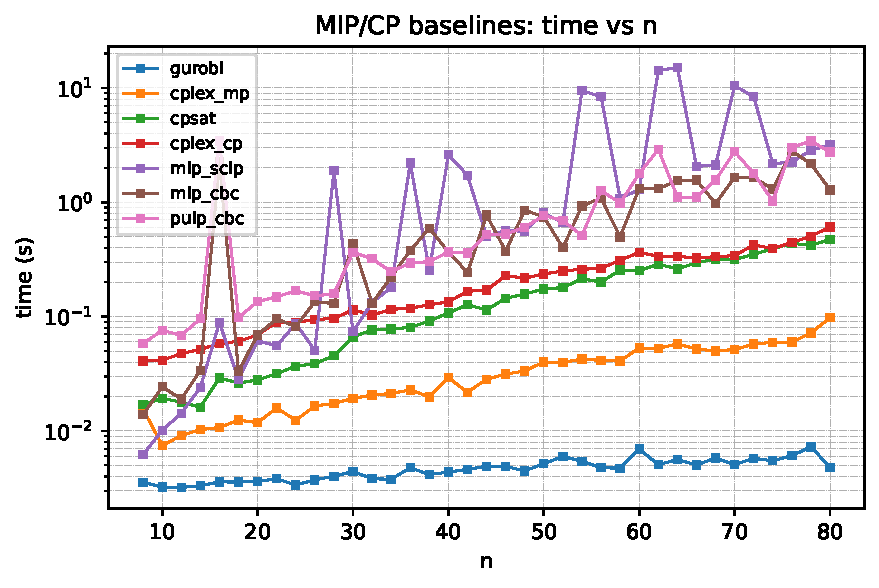
\includegraphics[width=\linewidth]{baselines_time_vs_n}
  \caption{Thời gian giải trung vị của các baseline MIP/CP theo $n$.}
  \label{fig:baselines}
\end{figure}

Hình~\ref{fig:comparison} so sánh cấu hình SAT tốt nhất (encoding binary với
MiniSat) với tất cả baseline. Với $n\geq 60$, phương pháp SAT tốt nhất vào khoảng
$0{,}3$--$0{,}9$\,giây, ngang ngửa CP-SAT và CPLEX CP và nhanh hơn rõ rệt các
baseline CBC/SCIP, nhưng chậm hơn CPLEX MIP và chậm hơn nhiều so với Gurobi.
Khoảng cách với Gurobi mở rộng khi $n$ tăng.

\begin{figure}[t]
  \centering
  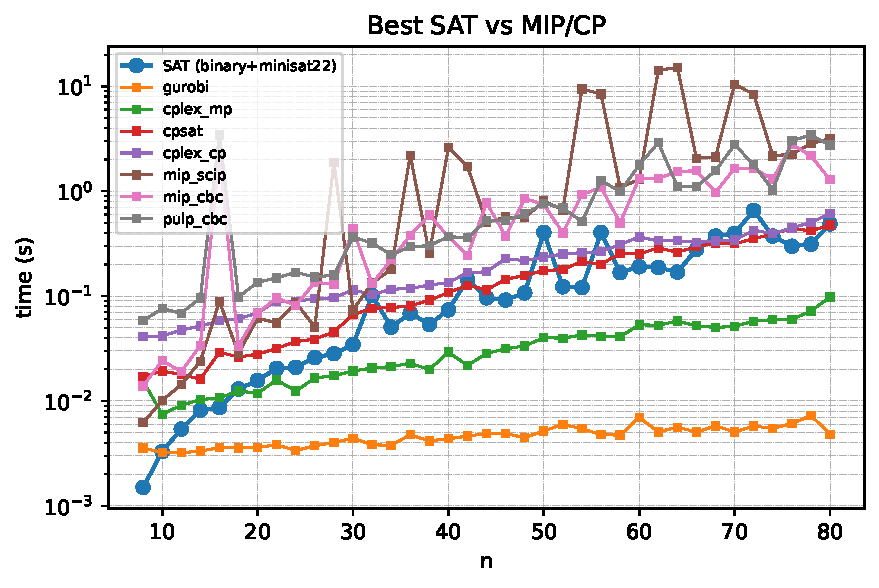
\includegraphics[width=\linewidth]{method_comparison}
  \caption{Cấu hình SAT tốt nhất (encoding binary với MiniSat) so với các baseline
  MIP/CP.}
  \label{fig:comparison}
\end{figure}

\subsection{Thảo luận}
Ba nhận xét nổi bật. Thứ nhất, tương tác encoding--solver cho thấy không thể đánh
giá chất lượng encoding một cách tách biệt: pairwise thắng với các solver lan
truyền yếu vì số mệnh đề lớn đem lại lan truyền mạnh, còn binary thắng với các
solver CDCL mạnh vì giữ công thức nhỏ. Điều này phù hợp với quan điểm cổ điển rằng
encoding tốt nhất phụ thuộc vào solver \citep{Prestwich2009}. Thứ hai, chúng tôi
quan sát một hiện tượng đặc thù của solver: với instance pairwise nhỏ $n=8$,
CaDiCaL báo cáo số quyết định, lan truyền và xung đột đều bằng không vì nó giải
instance hoàn toàn trong pha tiền xử lý, không vào vòng lặp tìm kiếm; do đó các bộ
đếm này chỉ đo công sức tìm kiếm chứ không đo toàn bộ công việc. Điều này khẳng
định rằng thống kê dựa trên lan truyền cần được dùng cẩn trọng khi so sánh các
solver khác loại. Cuối cùng, bộ giải MIP thương mại Gurobi chiếm ưu thế trước mọi
phương pháp chính xác khác trên bài toán mang tính khả thi này, cho thấy với
instance khả thi nhỏ, tiền xử lý và heuristic của MIP được tinh chỉnh có thể vượt
qua một quy trình SAT tổng quát dù được mã hoá cẩn thận. Ưu thế của SAT nằm ở tính
mô-đun: cùng một mô hình chạy được với nhiều solver và encoding, và cấu hình tốt
nhất vẫn cạnh tranh với CP-SAT và CPLEX CP.

\section{Kết luận}\label{sec:conclusion}
Chúng tôi đã trình bày một phương pháp mã hoá SAT chính xác cho N-Queens, cài đặt
với năm cách mã hoá đếm tự viết và bảy cách của PySAT cùng tám bộ giải SAT, và so
sánh với bảy baseline MIP/CP. Thực nghiệm cho thấy tương tác mạnh giữa encoding và
solver, chỉ ra MiniSat và MiniCard là các solver hiệu quả nhất cùng pairwise và
binary là các encoding tốt nhất tuỳ theo solver, và khẳng định sức mạnh của MIP
thương mại trên bài toán này. Hướng phát triển gồm mở rộng sang biến thể tối ưu
của N-Queens (tối đa số quân hậu trên bàn $n\times m$), sang các instance vô nghiệm
khó hơn, và bổ sung thêm solver khi các solver bị crash và thiếu trở nên khả dụng.

\section*{Tuyên bố về việc sử dụng AI tạo sinh trong quá trình chuẩn bị bản thảo}
Trong quá trình chuẩn bị công trình này, tác giả đã sử dụng một mô hình ngôn ngữ
lớn để hỗ trợ gỡ lỗi mã nguồn, soạn thảo văn bản và hiệu đính ngôn ngữ. Sau
khi sử dụng công cụ này, tác giả đã xem xét và chỉnh sửa nội dung khi cần và chịu
hoàn toàn trách nhiệm về nội dung của công trình.

\bibliographystyle{cas-model2-names}
\bibliography{../refs}

\section*{Dữ liệu nghiên cứu}
Mã nguồn, dữ liệu benchmark và các script tái tạo toàn bộ hình và bảng có tại:
\begin{center}
\url{https://github.com/Duc-2705/n-Queens}
\end{center}

\end{document}
